\chapter{Validity of TRACS results for irradiated silicon detectors}

It has already been discussed the theoretical basis upon which TRACS has been developed to include radiation damage effects into its simulations. It has also been discussed how those implementations were made. Now all that is left for TRACS to be considered a useful tool in research. Just like any tool to be used in research, TRACS needs to be consistent with experimental results or, as we are talking about a simulation tool, be able to reproduce reliably experimental results.

%here p``olsen
A first way to attest the validity of TRACS results after the implementation of radiation damage is to compare them to other measurement already published and accepted results from other simulators. In the thesis published by T.P\"{o}lsen in 2010 it is shown how a linear parametrisation of the \neff can e used to reproduce laboratory measurements accurately. 

These results will be used as the first test to check how accurately TRACS can reproduce real world conditions in its simulations. It is also necessary to conduct a controlled test in which TRACS is compared against real data measured in the laboratory. By doing this the author can attest the validity of the measuring and simulation procedures. This task will be the second and last test to validate TRACS results.

TRACS is able to reproduce any kind of TCT measurement provided an accurate input of carrier distribution inside the detector. To perform the comparison it is needed to chose one of the three previously mentioned TCT techniques. The SSD group at CERN has in its facilities setups that allow researchers to perform both red-TCT and edge-TCT measurements with a good level of automation. Due to availability of measuring schedule, the choice was made to perform red-TCT measurements in the TCT+ setup at the aforementioned SSD group at CERN, to be compared with simulations from TRACS. In particular bottom-TCT was chose after several measurements for it was the one that showed clearly the signs of radiation damage in the form of the \textit{Double Peak} as a result of the \textit{Double Junction} explained in section \ref{sec:rad}. 

It is important to note that TRACS needs to be given between 3 and 7 different parameters to perform a correct simulation of an irradiated silicon detector. This complexity call for automated fitting software to perform parameter selection to match TRACS simulation to the experimental results. Such a software is planned to be developed but it is not available at the time of writing this report. It is for this reason that comparison with real-world measurements will only be performed with one detector and one technique. Selection and optimisation of the previously mentioned parameters that TRACS require to perform a simulation of irradiated silicon detector will be done manually by trial-and-error. Such parameters are not expected to be quantitatively accurate due to the complexity of the fitting process. The simulation-measurement comparison is, hence, not intended as categorical proof of TRACS accuracy but rather as a showcase of TRACS newly implemented characteristics; namely reproduce the features of the transients generated by irradiated silicon detectors.

To avoid adding more sources of complexity to the simulation, the detector used was the most simple silicon detector: a diode. The diode had been previously irradiated with a fluence of $\PHI = 10^{15} neq$. It has a standard diode geometry of 1cmx1cm surface with 300 $\mu$m width with a structure similar to that explained in section \ref{REFERENCIA A DEFINIR}. The diode was also subject to the standard annealing process after irradiation and stored in a fridge to ensure constant low temperatures and prevent radiation effects to grow over time. This also complies with the standard irradiation-storage-measurement procedure that is followed in most of the research experiments on radiation damage in silicon detectors.

In the following sections an extended description of the experimental setup and  measurement procedure will be presented, followed by a discussion of the results and the comparison between TRACS simulations and laboratory measurements.

\section{Data acquisition process} % (fold)
\label{sec:future_improvements}

To compare TRACS to previous simulations the process is straight forward. The only steps needed to be taken were gathering the data from previous simulations and reproducing the plots using TRACS and the same linear \neff parametrisation used in the reference simulation. The only unusual step taken was the digitalization of the plots presented in the referenced thesis so that comparison in the same plot was possible. For the rest of this section we will focus only on the TCT techniques and the setup and measuring procedure in the laboratory for it was performed by the author as part of this project.

The basics of TCT measurement techniques have been explained in section \ref{sec:tct} so this section will focus on the more specific implementation of those principles of operation in the TCT+ setup at CERN. The TCT+ setup is a standard laboratory setup belonging to the SSD group in which this project was developed. The measurements were performed by the author using the previously mentioned facility under supervision of a member of the SSD group. Therefore the details explained in the following subsections will be specific to the TCT+ setup as used by the SSD group at CERN. However, since most of the components and arrangement of TCT+ are similar to those used in most of the TCT-capable facilities, many of the explanations ahead will be applicable to any TCT setup elsewhere. 

Explanation of the experimental procedure will be presented after setup description. The procedure that will be described also falls under the same considerations as TCT+ setup, since it will also be specific to the particular measurement performed for this project but will be applicable for any TCT measurement almost entirely. 

The process of adjusting the parameters for the simulation to match the measurements will also be commented, albeit briefly. The fitting of the simulations will be performed in a purely trial-an-error manner and is not of much interest for the project as software is expected to be available to perform such task in a more efficient manner. 

%To perform the bottom-TCT measurements For a silicon detector to be used as so, it is needed to have a circuit that can apply the necessary \vias and read the signal as well as a mechanism to generate free carriers inside the silicon bulk (e.g.: particles or laser). In this section we will explain in detail how these things are set-up together for performing controlled, reliable measurements in the laboratory.

\subsection{Setup} % Necesita un buen repaso

In the first place, the components of the circuit that are required must be stated. The list contains a power supply for applying the \vias, a Resistor-Capacitor system for signal filtering and an amplifier for improving Signal to Noise ratio. An Oscilloscope was also used as measuring device for it has fast response and enough resolution to measure the signal coming from the silicon diode.

The RC system and the Amplifier are placed right after the detector (following the direction of flow of the current). The Oscilloscope or measuring device is positioned at the end, as shown in the sketch below this lines REFERENCE HERE TO IMAGE! Even though these placements decisions are fairly trivial it is important to understand what the role of each component in the circuit is.

By looking at the figure REFERENCE AGAIN!!!! it is easier to understand what each of the components is doing and why it is so important to have such a configuration even for the most basic setups. The purpose of having an RC device is to separate the DC component (\vias) from the AC component (signal from the detector) of the total signal that would be otherwise collected at the readout point. By using a Resistor-Capacitor system the \vias and the signal gets separated allowing for the use of an amplifier that would be effective, since \vias is typically over several hundred volts and the amplifiers used do not accept more than 5V. This separation not only allows for the small signal to be amplified but also allows for better S/N ratios 

The reason why the RC system and the amplifier appear boxed together in the sketch is that they usually are part of the same device called \textit{Bias Tee} (due to its shape and the fact that is used for applying bias voltages on silicon detectors). From the amplifier the signal will be read by the oscilloscope connected to it. The oscilloscope is usually set to average a couple of hundreds of signals for smoother and cleaner waveforms as well as to eliminate random fluctuations.The signal is then stored and analysed with the corresponding software, depending on the parameters of interest.

Once it has been discussed how the circuit is setup for measurements it is time to focus on some consideration that need to be taken into account to ensure the reproducibility and reliability of the results; mainly related to eliminate noise from the signal. These precautions are standard in any TCT measurement and when they are correctly carried out, they ensure the signal that is read is  only the signal coming from the detector and only due to the carriers created by the laser illuminating the detector.

Isolation of the system from outside sources of signal is performed in two main ways: isolation from external light sources and isolation from electromagnetic external signals. For the first of the two tasks it suffices to work in a dark environment. Since electron-hole pairs in silicon are created only by photons in the near infrared or higher energies, it is only necessary that the visible and near infrared be blocked to ensure that all the carriers generated in the silicon come only from the light of the laser used in the experiment.

To insulate the setup from any electromagnetic signals coming from outside sources the most common and widespread solution is to enclose the laser and detector inside a Faraday cage. Faraday cages are easy and cheap to build and provide the needed electromagnetic insulation to ensure the signal read in the experiments is coming only form detector and has no interference (noise) component or (in the real case) as little as possible. Since cable need to be passed through the Faraday cage, it is never possible to build a perfect Faraday cage and have total insulation. In the real case cables coming in and out of the box acting as a Faraday cage need to be properly insulated, to ensure enough EM insulation.

To create signal inside the detector, laser illumination is used. Laser provide and easily controllable light source that has a very repeatable behaviour, ideal for laboratory experiments. The laser used in this particular experiment is a red laser with wavelength $\lambda = 660nm$ with other TCT techniques require of different wavelengths and laser properties. The associated photon energy of the red laser used in our experiment ($E_{red} \approx 1.88 eV$) is above the required energy to promote electrons from the valence band to the conduction. Photons coming from the red laser are able to create electron-hole pairs on their own, so charge carriers of both signs will be created inside the detector insofar as the beam can penetrate inside the detector which for red light is of the order of a few $\mu m$, as we have previously mentioned in section \ref{sec:tct}

The detector is then mounted on motorised servo controllers that can change the detector position with respect to the laser beam with micrometric precision. In TPA and edge TCT measurements these servo controllers are used to effectively move the laser inside the detector when performing different types of scans. In the case of red-TCT they are equally important but only used to align the detector window with the laser beam. For bottom-TCT measurements it is not really critical where the laser illuminates the detector as long as it is not reflected on the metal frame. Since the diode has a very simple geometry, almost any part of the detector behaves the same for red illumination. The only requirement for consistency being that the beam should be completely inside the window opened in the metalisation part of the diode specifically for that purpose.

Temperature is very important when measuring silicon detectors, not only because it can accelerate radiation damaging but also because the mobility of electrons and holes is dependant on such magnitude. To make sure the temperature of the silicon detector remains constant throughout the experiment, a Peltier device is used. Peltier devices exploit Peltier effect to change their temperature at very fast rates. They are commonly used in TCT measurements for both temperature control and temperature change. In the measurement performed for the project it was used for both purposes with a target temperature of $T = -100C \approx 170K$ during all the measurements.

\subsection{Experimental procedure} 

The measuring procedure itself is fairly simple but there are some preparation steps that need to be carried out to ensure good results. Once everything has been set up correctly and re-checked one can proceed to operate. First critical point to cover is to align the laser beam with the window in the diode. To perform the alignment efficiently a good starting point is of good help. One of the techniques to find the window is to look at the live signal coming form the detector with a $ \vias \beq V_{dep}$ and perform a full coarse scan on one of the axis (X or Y) waiting for the transient to appear. If $V_{dep}$ a quick approximation of its value should be enough to use this method successfully\footnote{For bottom-TCT the approximation should underestimate $V_{dep}$ to ensure full depletion of the volume when searching for the window, otherwise no signal will be read}. During the scan it should be easy to pick-up when the device reads some signal from the detector; at this point the laser beam is, at least partially, inside the window. From them on it is only a matter of using finer adjustments to reach the maximum signal possible. Both servo controllers should be used in this step to make sure the beam is not being partially blocked by the edge of the window. Once the maximum in the signal has been found, the servo controllers should remain in the same position throughout the whole data-taking process.


With alignment performed the data acquisition process is straight forward. In the software used to control the TCT+ setup allows for automatic stepping up of the \vias applied to the detector. It is only necessary to configure the software with the correct voltage step (in our case we chose $\DELTA \vias = 10V $) and also the maximum and minimum voltages (we chose $-10 \leq \vias \beq 500$ ). The software will then take control of the setup and record one waveform for each of the different \vias values set in the loop. The TCT+ setup can also be configured to move modify the detector position in a similar way to that of the voltage, but for a measuring a diode using red-TCT technique it is not interesting such an option. It is also important to note that the waveform recorded and store by the TCT+ software is the average of many of them as previously stated. In our case it was decided to average over 256 waveforms.

The recorded data is stored in a plain text file following a specific format designed for the SSD group. This files are specifically designed to be analysed using the software developed at the SSD group for that purpose. This helps standardise data analysis routines amongst the group and improves efficiency as software is shared amongst the whole group. The waveforms are plotted and some, selected for direct comparison with TRACS simulation results. The selection criteria will be to find the most representative waveforms that show those features characteristic of irradiated silicon detectors, such as the DP coming form the DJ. 

It has been stated before, but it is important to remember that the comparison will only be done in terms of qualitative similarity and no exhaustive quantitative analysis will be perform. The reason for this uncommon comparison being the complexity of the fitting processed that requires 7 parameters to be estimated for the simulation. It is reasonable to suppose that if a trial-an-error manual fit can mimic qualitatively the features present in a real world measurement, an automated fitting process could do a much better job. In this case one can assume that the discrepancy between the simulations and the measurements is not due to faults in the software but to a poor fitting method as it is the one used in this particular case.  

\section{Results and comparison} % (fold)
\label{sec:comparison}

The data has been normalised to the maximum value of the histograms. In this way the direct comparison is easier while any disagreement in the laser illumination part is eliminated. Comparison will be presented in two different manners. First a comparison of each set of data (measurements and simulations) will be presented in separated plots. This will illustrate similarities in the trends followed by the transients when \vias is increased.

A few sample transients will be selected for direct comparison between measurements and simulations. Simulation and measurements will be plotted together with different plots for each of the selected voltages. This will allow to compare the specific features of the transients and establish the agreement between simulations and measurements.

\subsection{Comparison between TRACS and already existing simulations}

The first milestone for TRACS is to reproduce already published and approved results that other simulators have achieved. For such task the data from [ref{REFERENCIA A DECIDIR}] will be used. In this thesis, the \neff is parametrised as a linear function of depth, a feature TRACS also bares. Even though the data is not available in any other form than the plots published in the aforementioned thesis, it is possible to extract the defining parameters of the \neff and perform a simulation that can be compared to the published one. 

Transients from T.P\"{o}hlsen's thesis also include measured data that supports the validity of the simulation presented there, but the estimated \neff used to generate the \vec{E} fields and transients was not measured in the laboratory but fitted from the transients' shape. The values extracted from the plot in the reference for the \neff were $\neff(z = 0) = 2.5 \cdot 10^{13} cm^{-3}$ and $\neff(z = 150) = -5 \cdot 10^{13} cm^{-3}$. From such parameters we can define a linear \neff distribution in TRACS and the results we obtained for the \vec{E} field are presented in Figure \ref{fig:CompFields}

\begin{figure}[H]
	\centering
	Aqui deberian estar los fields Pohlsen y TRACS comparados
	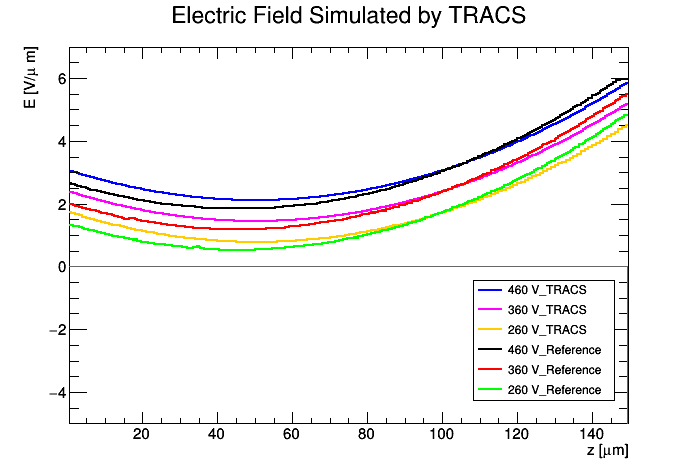
\includegraphics[width=0.8\textwidth]{Pohlsen_fields.png}
	\label{fig:CompFields}
	\caption{Electric field inside the diode as a function of depth. Simulations from [REFERENCIAPOHLSEN] and TRACS are plotted together for comparison. Agreement between both simulations is remarkable}
\end{figure}

\begin{figure}[H]
	\centering
	Esto desaparecera cuando junte los plots
	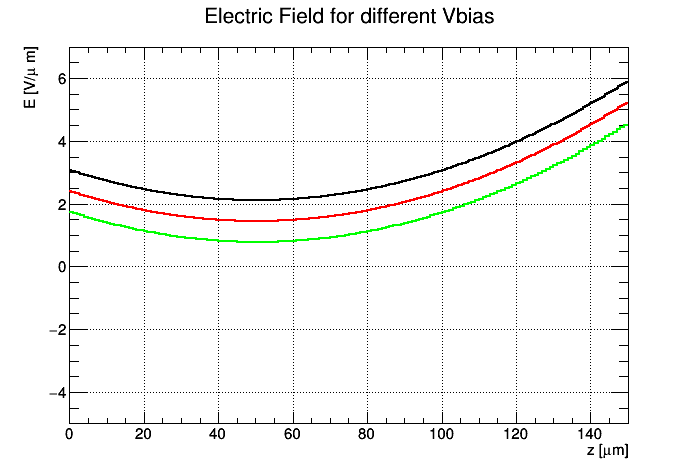
\includegraphics[width=0.88\textwidth]{TRACSpohlsFields.png}
	\label{fig:mues2}
	\caption{Imagen of the detected wavefront for the laser without any aberration introduced. The values are: $P2V = -0.055waves$ and $P = 0.001D$. Anything below those values is considered noise.}%referenciar en el pie de figura
\end{figure}

Now top-TCT was simulated and the obtained transients compared to the laboratory measurements. The same simulations were performed with TRACS and compared to the simulations and measurements from the reference. It is important to note that the trapping simulation is different between both simulators with TRACS having a constant $\tau$ whilst the reference uses a field-dependant $\tau$. Results are therefore expected to not me the same but compatible.

\begin{figure}[H]
	\centering
	Aqui deberian estar los transients Pohlsen y TRACS comparados
	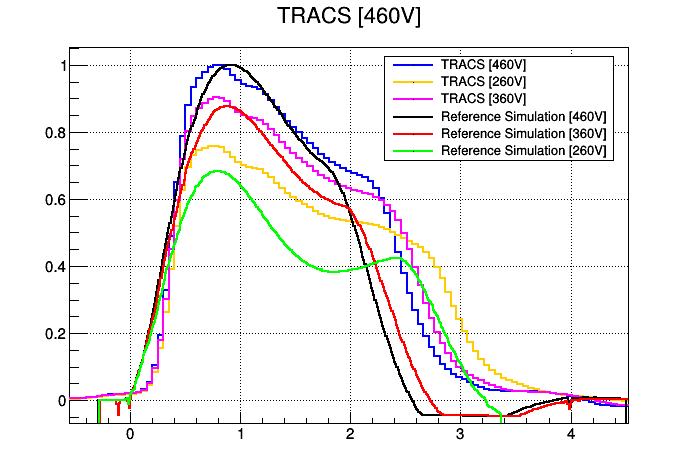
\includegraphics[width=0.8\textwidth]{Pohlsen_scr.png}
	\label{fig:mues2}
	\caption{Transient currents generated by top-TCT measurements and simulations. TRACS uses a different trapping parametrisation yielding slightly different results while maintining the general features of both measurements and simulations from [REFERENCIAPOHLSEN]}
\end{figure}

\begin{figure}[H]
	\centering
	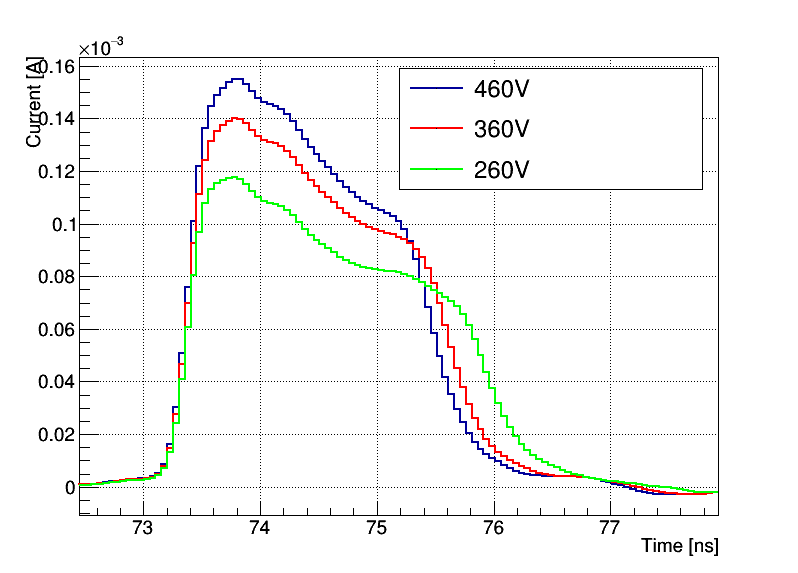
\includegraphics[width=0.88\textwidth]{Pohlsen.png}
	\label{fig:mues2}
	\caption{Imagen of the detected wavefront for the laser without any aberration introduced. The values are: $P2V = -0.055waves$ and $P = 0.001D$. Anything below those values is considered noise.}
\end{figure}

\subsection{Comparison between simulations and real world measurements}

%Deberia haber comentado en la parte de TRACS sobre que TRACS no simula difusion?

In order to reproduce the transients obtained in the laboratory the trial-and-error method was performed manually. The results presented in this section are considered to be a good representation of the measured detector but by no means a perfect match, as previously mentioned. The chosen \neff parametrisation was the Trilinear form for TRACS is the only simulator that can perform such parametrisation. A table with the 8 defining values for the chosen \neff are presented below together with a plot of the \neff distribution as a function of depth. Trapping constant was chosen to be: $\tau = 5 ns$



Measured data is presented now. In the following plot all the transients measured in the laboratory can be seen together. It can be seen that the Double Peak feature appears only for $\vias \geq 80 V$. This value of \vias can be considered a good estimation of the $V_{dep}$. It can be seen that transients get shorter in time with increasing voltages with the second peak getting higher with higher voltages. 

\begin{figure}[H]
	\centering
	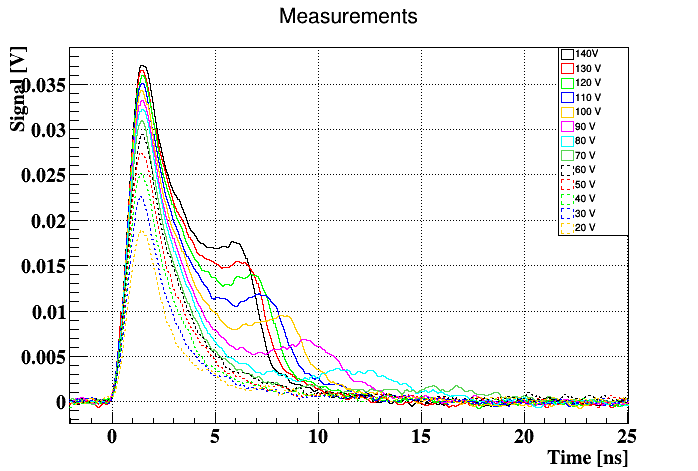
\includegraphics[width=0.9\textwidth]{c1.png}
	\label{fig:mues2}
	\caption{Imagen of the detected wavefront for the laser without any aberration introduced. The values are: $P2V = -0.055waves$ and $P = 0.001D$. Anything below those values is considered noise.}
\end{figure}
				
TRACS simulations are presented now in a similar manner as the measurements. Comparison of the transient response to higher voltages can be done with these plots. It can be seen that TRACS simulations follow a similar trend of shorter transients and higher second peaks with increasing voltages.

\begin{figure}[H]
	\centering
	\centering
	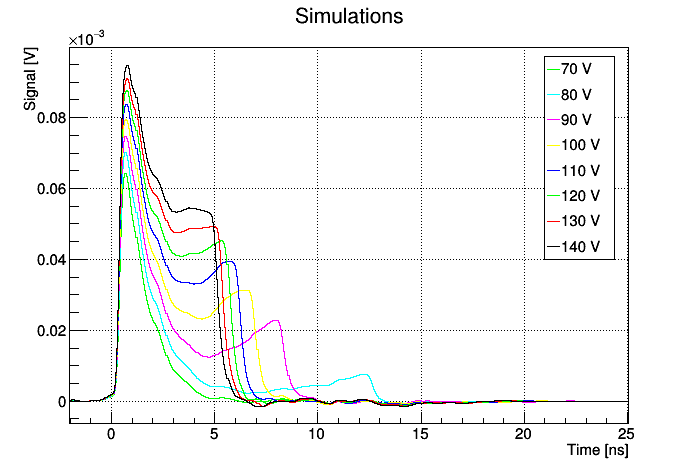
\includegraphics[width=0.9\textwidth]{AllSims.png}
	\label{fig:mues2}
	\caption{Imagen of the detected wavefront for the laser without any aberration introduced. The values are: $P2V = -0.055waves$ and $P = 0.001D$. Anything below those values is considered noise.}
\end{figure}

No transients below $80V \approx V_{dep}$ were simulated because TRACS does not simulate diffusion inside the detector. Together with the fact that illumination is done in the non depleted area for $V < 80V$ this means that any simulation done in TRACS for voltages under $V_{dep}$ will have no physical meaning.

These two plots allow to see how TRACS reproduces the trends of the transients with different voltages but direct comparison of the transients can be arduos. In the following plots a direct comparison of selected transients will be presented for a more comprehensive look at the transient features and how TRACS is able to simulate real world measurements.

From the previous voltage scans, three transients have been selected. The three voltages selected are 80V, 100V and 140V. The lowest values was selected because it's the lowest value at which the Double Peak feature is visible, the highest voltage was chosen for that particular reason and 100V will be shown to have a point in between those maximum and minimum values.

\begin{figure}[H]
	\centering
	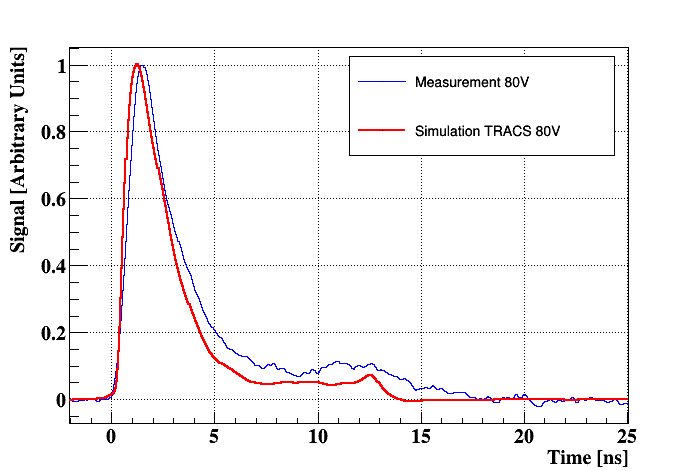
\includegraphics[width=0.9\textwidth]{80V.png}
	\label{fig:mues2}
	\caption{Imagen of the detected wavefront for the laser without any aberration introduced. The values are: $P2V = -0.055waves$ and $P = 0.001D$. Anything below those values is considered noise.}
\end{figure}

\begin{figure}[H]
	\centering
	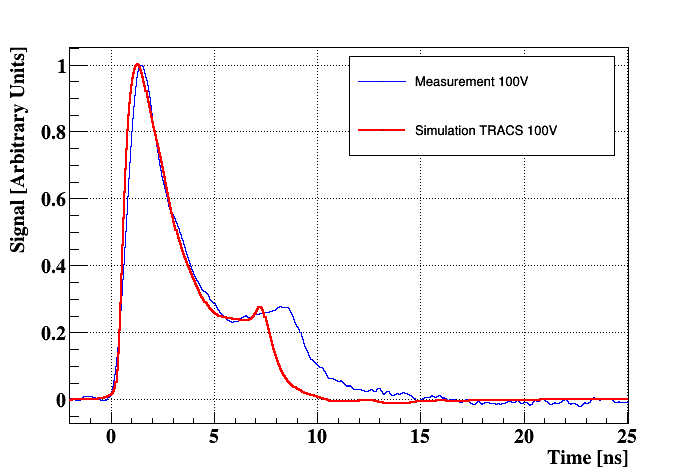
\includegraphics[width=0.9\textwidth]{100V.png}
	\label{fig:mues2}
	\caption{Imagen of the detected wavefront for the laser without any aberration introduced. The values are: $P2V = -0.055waves$ and $P = 0.001D$. Anything below those values is considered noise.}
\end{figure}

\begin{figure}[H]
	\centering
	\includegraphics[width=0.9\textwidth]{140V.png}
	\label{fig:mues2}
	\caption{Imagen of the detected wavefront for the laser without any aberration introduced. The values are: $P2V = -0.055waves$ and $P = 0.001D$. Anything below those values is considered noise.}
\end{figure}

Looking at the three comparison figures it is easy to see that TRACS simulations show tha same features and behaviour as the real measurements. The fact that the simulations don't match perfectly the measurements can be attributed to the electrnoics shapping algorithm (the transfer function of the amplifier used in the measurements was not available for the simulations) and also to the only approximate fitting of the parameters, as we have discussed before. Better agreement between simulations and measurements can be expected if this problems are addressed.
% section future_projection (end)

To-Do:

- Decide how to show plots
- Fix Plots
- Fix References (BibTex)
- Get Neff plot

